\documentclass[10 pt,usenames,dvipsnames, oneside]{article}
\usepackage{../../../modelo-ensino-medio}



\begin{document}

\begin{center}
  \begin{minipage}[l]{3cm}

\includegraphics[width=2cm]{logo}    
\end{minipage}\hfill
\begin{minipage}[r]{.8\textwidth}
 {\Large \scshape Atividade: Locadora de carros}  
\end{minipage}
\end{center}
\vspace{.2cm}

\ifdefined\prof
%Habilidades da BNCC
% \begin{objetivos}
% \item 
% \end{objetivos}

%Caixa do Para o Professor
\begin{goals}
%Objetivos específicos
\begin{enumerate}
\item Reconhecer o significado geométrico das desigualdades.
 \item Estabelecer conexão entre o conceito de desigualdade e sua simbologia matemática.
\end{enumerate}

\tcblower

%Orientações e sugestões
\begin{itemize}
\item Nessa atividade, pretende-se levar o aluno a perceber a relação entre a expressão “menor que” e o símbolo matemático $<$, bem como identificar uma representação gráfica da solução de uma inequação.
\item Incentive seus alunos a escrever as respostas tanto em termos literais (usando palavras) quanto em termos matemáticos (usando a notação matemática).
\end{itemize}
\end{goals}

\bigskip
\begin{center}
{\large \scshape Atividade}
\end{center}
\fi

Atualmente existem diversas locadoras de veículos, permitindo uma concorrência saudável para o mercado, fazendo com que os preços se tornem acessíveis. Nas locadoras \emph{Possante} ($P$) e \emph{Qualicarro} ($Q$), o valor da diária de seus carros depende da distância percorrida em km, conforme o gráfico abaixo:

\begin{figure}[H]
\centering
\noindent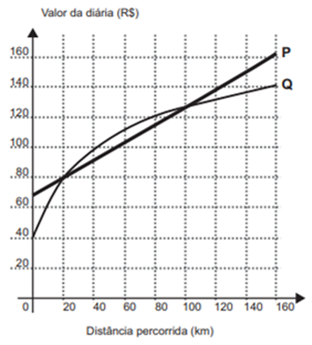
\includegraphics[width=180bp]{locadora}
\end{figure}


\begin{enumerate}

\item{}
Suponha que uma pessoa resolveu alugar um carro pela locadora $Q$ e pagou menos que 100 reais pelo valor da diária. Quais os valores possíveis para a distância que essa pessoa percorreu com o carro?

\item{}
Se um outro cliente alugar um carro, agora na locadora $P$ e pagar no mínimo 80 e no máximo 140 reais na diária do veículo, quais os possíveis valores para a distância percorrida com ele?

\item{}
Qual a locadora mais vantajosa, em termos de custo do aluguel, para uma pessoa que deseja alugar um carro para percorrer uma distância total de $80 km$?

\item{} Para quais valores da distância a ser percorrida de carro por uma pessoa, o custo do aluguel será o mesmo tanto para a locadora $P$ quanto para a $Q$?

\item{} Para quais valores da distância a ser percorrida de carro por uma pessoa, fica mais barato alugar o carro pela locadora $P$. E pela locadora $Q$? 

\end{enumerate}

\ifdefined\prof
\begin{solucao}

\begin{enumerate}
\item Até $40$ km.
\item Distâncias entre $20$ km e $120$ km.
\item A locadora $P$.
\item  $20$ km e $100$ km. 
\item Locadora $P$: entre $20$ km e $100$ km.
Locadora Q: de $1$ km a $20$ km ou distâncias superiores a $100$ km.
\end{enumerate}

\end{solucao}
\fi

\end{document}